\documentclass[10pt,a4paper]{article}

% ==============================================================================
% IOT LABORATORY: MASTER PRINTABLE CODE & OUTPUTS BOOKLET (EXPERIMENTS 01 - 06)
% Formatted with 1.0-inch lateral margins, high readability, and zero header/footers.
% Exactly 6 Self-Contained A4 Pages (1 Page per Experiment)
% ==============================================================================
\usepackage[utf8]{inputenc}
\usepackage[T1]{fontenc}
\usepackage{lmodern}
\usepackage[left=1.0in, right=1.0in, top=0.32in, bottom=0.32in]{geometry}
\usepackage{amsmath,amssymb}
\usepackage{xcolor}
\usepackage{listings}
\usepackage{graphicx}
\usepackage{tikz}
\usetikzlibrary{shapes.geometric,arrows.meta,positioning,calc}
\usepackage{booktabs}
\usepackage{tabularx}
\usepackage{titlesec}
\usepackage{caption}
\usepackage{microtype}
\usepackage{float}

\pagestyle{empty}
\setlength{\parindent}{0pt}

\titleformat{\section}
  {\normalfont\normalsize\bfseries\raggedright}{\thesection}{0.5em}{}[\titlerule]

\titlespacing*{\section}{0pt}{5pt}{2pt}

\lstdefinestyle{bwCode}{
    language=C++,
    basicstyle=\ttfamily\scriptsize,
    keywordstyle=\bfseries,
    commentstyle=\itshape,
    stringstyle=\ttfamily,
    numbers=left,
    numberstyle=\tiny,
    numbersep=5pt,
    stepnumber=1,
    breaklines=true,
    breakatwhitespace=true,
    frame=single,
    rulecolor=\color{black},
    tabsize=2,
    showstringspaces=false,
    columns=fullflexible,
    keepspaces=true,
    lineskip=-0.3pt,
    aboveskip=2pt,
    belowskip=2pt
}

\lstdefinestyle{bwTerminal}{
    basicstyle=\ttfamily\scriptsize,
    numbers=none,
    breaklines=true,
    breakatwhitespace=true,
    frame=single,
    rulecolor=\color{black},
    columns=fullflexible,
    keepspaces=true,
    lineskip=0.0pt,
    aboveskip=2pt,
    belowskip=2pt
}

\captionsetup{font=footnotesize,labelfont=bf,skip=2pt}

\begin{document}

% ==============================================================================
% PAGE 1: EXPERIMENT 01 - IOT ARCHITECTURE & MQTT TELEMETRY PAYLOAD
% ==============================================================================
\begin{center}
    {\large\bfseries Experiment 01: Overview of IoT Architecture \& Protocols}\\[0.06cm]
    {\normalsize\textbf{5-Tier Architecture, Protocol Comparison \& MQTT Telemetry Payload Code}}
\end{center}
\vspace{-0.24cm}
\rule{\textwidth}{0.8pt}
\vspace{0.06cm}

\section*{1. Constrained IoT Application Protocols Matrix}
\begin{table}[H]
\centering
\scriptsize
\setlength{\tabcolsep}{4.5pt}
\renewcommand{\arraystretch}{1.20}
\begin{tabularx}{\textwidth}{|p{1.8cm}|p{1.7cm}|p{3.2cm}|p{2.1cm}|X|}
\hline
\textbf{Protocol} & \textbf{Transport} & \textbf{Messaging Model} & \textbf{Header Size} & \textbf{Primary Application Domain} \\
\hline
\textbf{MQTT} & TCP (1883) & Publish / Subscribe & 2 Bytes (Fixed) & Real-time sensor telemetry, SCADA, battery-backed nodes. \\
\textbf{CoAP} & UDP (5683) & REST Request / Response & 4 Bytes (Fixed) & Constrained 8-bit MCUs, low-power lossy networks (LLNs). \\
\textbf{HTTP/REST} & TCP (80/443) & Client / Server Request & $>500$ B (Text) & Cloud-to-cloud APIs, enterprise REST integrations. \\
\textbf{WebSocket} & TCP (80) & Full-Duplex Stream & 2--10 Bytes & Live browser telemetry monitoring dashboards. \\
\hline
\end{tabularx}
\caption{Technical Comparison of IoT Application Layer Protocols.}
\end{table}

\vspace{-0.1cm}
\section*{2. Edge Microcontroller Telemetry Payload Firmware}
\begin{lstlisting}[style=bwCode, title={\textbf{Listing 1.1: Microcontroller Firmware for MQTT Telemetry Serialization.}}]
/*
 * Experiment 01: IoT Edge Telemetry Serialization & Protocol Ingestion
 * Formats multi-sensor readings into lightweight JSON payloads for MQTT Broker publishing.
 */

#include <ArduinoJson.h> // Standard lightweight embedded JSON library

void setup() {
  Serial.begin(9600); // Initialize UART Serial Interface
  Serial.println("==================================================");
  Serial.println("   IoT Lab: MQTT Node Telemetry Payload Stream   ");
  Serial.println("==================================================");
}

void loop() {
  // Step 1: Acquire mock sensory inputs from Perception Layer
  float currentTemp = 28.4;
  float currentHumidity = 62.5;
  int deviceUptime = millis() / 1000;

  // Step 2: Construct serialized JSON payload packet
  StaticJsonDocument<128> doc;
  doc["node_id"] = "ESP32_NODE_01";
  doc["uptime"]  = deviceUptime;
  doc["temp"]    = currentTemp;
  doc["hum"]     = currentHumidity;
  doc["status"]  = "ONLINE";

  // Step 3: Stream MQTT packet to Serial Gateway
  Serial.print("TOPIC: sensors/room1/telemetry | PAYLOAD: ");
  serializeJson(doc, Serial);
  Serial.println();

  delay(3000); // 3-second transmission cycle
}
\end{lstlisting}

\vspace{-0.1cm}
\section*{3. Simulated MQTT Broker Telemetry Stream Output}
\begin{lstlisting}[style=bwTerminal]
==================================================
   IoT Lab: MQTT Node Telemetry Payload Stream   
==================================================
TOPIC: sensors/room1/telemetry | PAYLOAD: {"node_id":"ESP32_NODE_01","uptime":3,"temp":28.4,"hum":62.5,"status":"ONLINE"}
TOPIC: sensors/room1/telemetry | PAYLOAD: {"node_id":"ESP32_NODE_01","uptime":6,"temp":28.6,"hum":62.1,"status":"ONLINE"}
TOPIC: sensors/room1/telemetry | PAYLOAD: {"node_id":"ESP32_NODE_01","uptime":9,"temp":28.9,"hum":61.8,"status":"ONLINE"}
TOPIC: sensors/room1/telemetry | PAYLOAD: {"node_id":"ESP32_NODE_01","uptime":12,"temp":29.1,"hum":61.5,"status":"ONLINE"}
\end{lstlisting}

\newpage

% ==============================================================================
% PAGE 2: EXPERIMENT 02 - DUAL ALTERNATING LED CODE & OUTPUT
% ==============================================================================
\begin{center}
    {\Large\bfseries Experiment 02: Interfacing Dual Alternating LEDs with Arduino UNO}\\[0.10cm]
    {\normalsize\textbf{GPIO Digital Output Control --- Program Source Code \& Circuit State Output}}
\end{center}
\vspace{-0.20cm}
\rule{\textwidth}{0.9pt}
\vspace{0.06cm}

\section*{1. Arduino C++ Source Code}
\begin{lstlisting}[style=bwCode, title={\textbf{Listing 2.1: Microcontroller Firmware for Periodic Anti-Phase LED Blinking.}}]
/*
 * Experiment 02: Dual Alternating LED Interfacing with Arduino UNO
 * Hardware Pin Connections:
 *   - Arduino Digital Pin 8 -> Green LED Anode (via 1 kOhm Resistor R1)
 *   - Arduino Digital Pin 7 -> Red LED Anode   (via 1 kOhm Resistor R2)
 *   - Common Ground (GND)   -> LED Cathodes
 * Switching Interval: 1000 ms (1.0 second periodic period)
 */
const int LED1_PIN = 8;    // Green LED Channel (Digital Pin D8)
const int LED2_PIN = 7;    // Red LED Channel   (Digital Pin D7)
const unsigned long BLINK_INTERVAL = 1000; // Period: 1000 ms (1.0 s)

void setup() {
  pinMode(LED1_PIN, OUTPUT); // Configure D8 as push-pull output driver
  pinMode(LED2_PIN, OUTPUT); // Configure D7 as push-pull output driver
  digitalWrite(LED1_PIN, LOW); // Initialize D8 LOW
  digitalWrite(LED2_PIN, LOW); // Initialize D7 LOW
}

void loop() {
  // Phase 1: LED1 ON (Active-HIGH 5V), LED2 OFF (Active-LOW 0V)
  digitalWrite(LED1_PIN, HIGH);
  digitalWrite(LED2_PIN, LOW);
  delay(BLINK_INTERVAL);
  // Phase 2: LED1 OFF (Active-LOW 0V), LED2 ON (Active-HIGH 5V)
  digitalWrite(LED1_PIN, LOW);
  digitalWrite(LED2_PIN, HIGH);
  delay(BLINK_INTERVAL);
}
\end{lstlisting}

\vspace{0.06cm}
\section*{2. Experimental Output, Logic Timing \& Truth Table}

\noindent
\textbf{A. Circuit State Truth Table \& Switching Log:}\par\vspace{0.06cm}
{\footnotesize
\setlength{\tabcolsep}{5pt}
\renewcommand{\arraystretch}{1.18}
\begin{tabularx}{\textwidth}{|c|c|c|X|}
\hline
\textbf{Interval} & \textbf{Pin 8 Output} & \textbf{Pin 7 Output} & \textbf{Observed Hardware State} \\
\hline
$0 - 1\,\text{s}$ & HIGH ($5\,\text{V}$) & LOW ($0\,\text{V}$) & \textbf{$\text{LED}_1$ ON}, $\text{LED}_2$ OFF ($I_{F1} \approx 3\,\text{mA}$, Green LED ON) \\
$1 - 2\,\text{s}$ & LOW ($0\,\text{V}$) & HIGH ($5\,\text{V}$) & $\text{LED}_1$ OFF, \textbf{$\text{LED}_2$ ON} ($I_{F2} \approx 3\,\text{mA}$, Red LED ON) \\
$2 - 3\,\text{s}$ & HIGH ($5\,\text{V}$) & LOW ($0\,\text{V}$) & \textbf{$\text{LED}_1$ ON}, $\text{LED}_2$ OFF (Periodic Alternation) \\
$3 - 4\,\text{s}$ & LOW ($0\,\text{V}$) & HIGH ($5\,\text{V}$) & $\text{LED}_1$ OFF, \textbf{$\text{LED}_2$ ON} (Periodic Alternation) \\
\hline
\end{tabularx}
}

\vspace{0.20cm}

\noindent
\textbf{B. Digital Timing Waveforms (Anti-Phase Switching, $T = 1.0\,\text{s}$):}\par\vspace{0.05cm}
{\centering
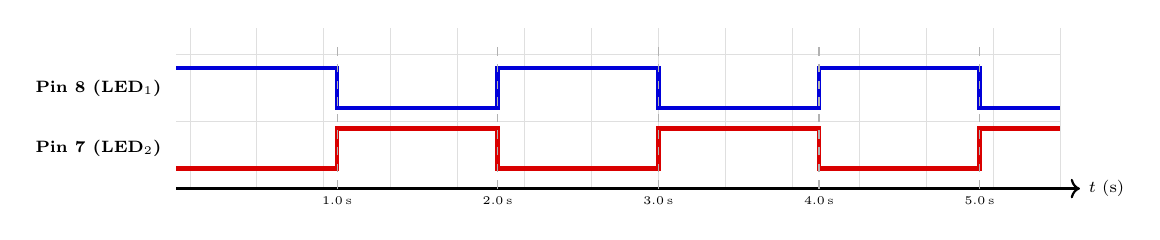
\begin{tikzpicture}[scale=0.85, every node/.style={transform shape}]
    \draw[step=1.0cm,gray!25,very thin] (1.8,0) grid (15.0,2.4);
    \draw[thick,->] (1.8,0) -- (15.3,0) node[right, font=\scriptsize] {$t$ (s)};
    
    % Pin 8 (LED1)
    \draw[ultra thick, blue!85!black] (1.8,1.8) -- (4.2,1.8) -- (4.2,1.2) -- (6.6,1.2) -- (6.6,1.8) -- (9.0,1.8) -- (9.0,1.2) -- (11.4,1.2) -- (11.4,1.8) -- (13.8,1.8) -- (13.8,1.2) -- (15.0,1.2);
    \node[left, font=\scriptsize\bfseries] at (1.7,1.5) {Pin 8 ($\text{LED}_1$)};

    % Pin 7 (LED2)
    \draw[ultra thick, red!85!black] (1.8,0.3) -- (4.2,0.3) -- (4.2,0.9) -- (6.6,0.9) -- (6.6,0.3) -- (9.0,0.3) -- (9.0,0.9) -- (11.4,0.9) -- (11.4,0.3) -- (13.8,0.3) -- (13.8,0.9) -- (15.0,0.9);
    \node[left, font=\scriptsize\bfseries] at (1.7,0.6) {Pin 7 ($\text{LED}_2$)};
    
    \foreach \x/\t in {4.2/1.0\,s, 6.6/2.0\,s, 9.0/3.0\,s, 11.4/4.0\,s, 13.8/5.0\,s} {
        \draw[dashed, gray!60] (\x,0) -- (\x,2.2);
        \node[below, font=\tiny] at (\x,0) {\t};
    }
\end{tikzpicture}\par\vspace{0.05cm}
{\small\textbf{Figure 2.1:} Digital logic anti-phase switching waveforms for complementary LED driving.}\par}

\newpage

% ==============================================================================
% PAGE 3: EXPERIMENT 03 - DHT11 SENSOR CODE & TELEMETRY OUTPUT
% ==============================================================================
\begin{center}
    {\large\bfseries Experiment 03: Interfacing DHT11 Sensor with Arduino UNO}\\[0.06cm]
    {\normalsize\textbf{Environmental Telemetry \& Alert Actuation --- Program Source Code \& Experimental Output}}
\end{center}
\vspace{-0.24cm}
\rule{\textwidth}{0.8pt}
\vspace{0.06cm}

\section*{1. Arduino C++ Source Code}
\begin{lstlisting}[style=bwCode, title={\textbf{Listing 3.1: Microcontroller Firmware for DHT11 Telemetry and Closed-Loop Alert Actuation.}}]
/*
 * Experiment 03: DHT11 Sensor Interfacing with Closed-Loop High-Temp Alert
 * Pin Connections: DHT11 DATA -> Pin 7 | Alert Red LED -> Pin 8 | 5V & GND -> Power
 * Alarm Trigger Threshold: 30.0 deg C (Adjustable setpoint)
 */
#include <DHT.h>

#define DHTPIN 7            // DHT11 DATA connected to Digital Pin 7
#define DHTTYPE DHT11       // Sensor model designation
#define ALERT_PIN 8         // Red Alert LED connected to Digital Pin 8
#define TEMP_THRESHOLD 30.0 // Closed-loop alarm trigger setpoint in Celsius

DHT dht(DHTPIN, DHTTYPE);

void setup() {
  Serial.begin(9600);
  pinMode(ALERT_PIN, OUTPUT);
  digitalWrite(ALERT_PIN, LOW); // Initialize alert LED to OFF
  dht.begin();
  Serial.println("=================================================");
  Serial.println("   IoT Lab: DHT11 Telemetry & Alert System       ");
  Serial.println("=================================================");
  Serial.println("Time(s)\tHumidity(%)\tTemp(C)\tAlert Status");
}

void loop() {
  delay(2000); // DHT11 1 Hz sampling rate constraint (2.0s polling interval)
  float humidity = dht.readHumidity();
  float temperature = dht.readTemperature();

  // Validate sensor readout frame
  if (isnan(humidity) || isnan(temperature)) {
    Serial.println("ERROR: Failed to read from DHT11 sensor!");
    return;
  }
  // Closed-Loop Threshold Comparison Logic
  bool isAlert = (temperature >= TEMP_THRESHOLD);
  digitalWrite(ALERT_PIN, isAlert ? HIGH : LOW);

  // Stream formatted telemetry to Serial Monitor
  Serial.print(millis() / 1000);
  Serial.print(" s\t");
  Serial.print(humidity, 1);
  Serial.print(" %\t\t");
  Serial.print(temperature, 1);
  Serial.print(" C\t");
  Serial.println(isAlert ? "ACTIVE [ALERT ON]" : "NORMAL [OFF]");
}
\end{lstlisting}

\vspace{0.06cm}
\section*{2. Experimental Output \& Serial Monitor Telemetry}

\noindent
\textbf{A. Temperature \& Humidity Measurement Matrix:}\par\vspace{0.06cm}
{\footnotesize
\setlength{\tabcolsep}{6pt}
\renewcommand{\arraystretch}{1.18}
\begin{tabularx}{\textwidth}{|c|p{4.2cm}|c|c|X|}
\hline
\textbf{\#} & \textbf{Thermal Specimen State} & \textbf{Temperature} & \textbf{Humidity} & \textbf{Actuator Alert State} \\
\hline
1 & Ambient Laboratory Air & $27.4^\circ\text{C}$ & $62.0\%$ & \textbf{OFF} (Temperature Below Setpoint) \\
2 & Ambient Laboratory Air & $28.1^\circ\text{C}$ & $60.5\%$ & \textbf{OFF} (Temperature Below Setpoint) \\
3 & Heated Thermal Transit & $31.8^\circ\text{C}$ & $74.0\%$ & \textbf{ON} (\textbf{High-Temp Alert Triggered}) \\
4 & Peak Heated State & $34.0^\circ\text{C}$ & $86.0\%$ & \textbf{ON} (\textbf{High-Temp Alert Triggered}) \\
5 & Stabilized Baseline & $28.5^\circ\text{C}$ & $65.0\%$ & \textbf{OFF} (Normalized Below $30^\circ\text{C}$) \\
\hline
\end{tabularx}
}

\vspace{0.22cm}

\noindent
\textbf{B. Serial Monitor Stream (9600 Baud):}\par\vspace{0.05cm}
\begin{lstlisting}[style=bwTerminal]
Time(s)    Humidity(%)    Temp(C)    Alert Status
2 s        62.0 %         27.4 C     NORMAL [OFF]
4 s        60.5 %         28.1 C     NORMAL [OFF]
6 s        74.0 %         31.8 C     ACTIVE [ALERT ON]
8 s        86.0 %         34.0 C     ACTIVE [ALERT ON]
10 s       65.0 %         28.5 C     NORMAL [OFF]
\end{lstlisting}

\newpage

% ==============================================================================
% PAGE 4: EXPERIMENT 04 - HC-SR04 ULTRASONIC SENSOR CODE & OUTPUT
% ==============================================================================
\begin{center}
    {\large\bfseries Experiment 04: Interfacing HC-SR04 Ultrasonic Sensor with Arduino UNO}\\[0.08cm]
    {\normalsize\textbf{Non-Contact Distance Measurement --- Program Source Code \& Experimental Output}}
\end{center}
\vspace{-0.22cm}
\rule{\textwidth}{0.8pt}
\vspace{0.08cm}

\section*{1. Arduino C++ Source Code}
\begin{lstlisting}[style=bwCode, title={\textbf{Listing 4.1: Microcontroller Firmware for Ultrasonic Distance Measurement.}}]
/*
 * Experiment 04: Ultrasonic Distance Measurement using HC-SR04 and Arduino UNO
 * Hardware Pin Connections:
 *   - Arduino Digital Pin 8 -> HC-SR04 TRIG (Trigger Output)
 *   - Arduino Digital Pin 7 -> HC-SR04 ECHO (Echo Pulse Input)
 *   - Arduino 5V & GND     -> HC-SR04 VCC & GND Power Supply
 * Serial Baud Rate: 9600 bps
 */
const int trigPin = 8;    // Pin D8 connected to HC-SR04 TRIG terminal
const int echoPin = 7;    // Pin D7 connected to HC-SR04 ECHO terminal

long duration;            // Holds raw Time-of-Flight (ToF) in microseconds
int distance;             // Holds calculated one-way distance in centimeters

void setup() {
  pinMode(trigPin, OUTPUT);  // Configure Trigger pin as digital output
  pinMode(echoPin, INPUT);   // Configure Echo pin as digital input
  Serial.begin(9600);        // Initialize UART Serial Interface at 9600 Baud
}

void loop() {
  // Step 1: Ensure a clean LOW signal before generating trigger pulse
  digitalWrite(trigPin, LOW);
  delayMicroseconds(2);
  // Step 2: Transmit 10 microsecond Active-HIGH Trigger Pulse
  digitalWrite(trigPin, HIGH);
  delayMicroseconds(10);
  digitalWrite(trigPin, LOW);
  // Step 3: Measure HIGH pulse duration on ECHO pin (Time-of-Flight in us)
  duration = pulseIn(echoPin, HIGH);
  // Step 4: Calculate one-way distance in centimeters (Speed of sound = 0.034 cm/us)
  distance = duration * 0.034 / 2;
  // Step 5: Format and stream telemetry data to Serial Monitor
  Serial.print("distance : ");
  Serial.println(distance);
  // Step 6: Measurement cycle delay to prevent acoustic multipath echo interference
  delay(100);
}
\end{lstlisting}

\vspace{0.06cm}
\section*{2. Experimental Output \& Serial Monitor Telemetry}

\noindent
\textbf{A. Ultrasonic Distance Measurement \& Calibration Log:}\par\vspace{0.06cm}
{\footnotesize
\setlength{\tabcolsep}{6pt}
\renewcommand{\arraystretch}{1.18}
\begin{tabularx}{\textwidth}{|c|c|c|X|}
\hline
\textbf{Trial} & \textbf{Actual Range} & \textbf{Serial Output} & \textbf{Measurement State \& Hardware Observation} \\
\hline
1 & $5.0\,\text{cm}$ & \texttt{distance : 5} & Exact Setpoint Match ($100\%$ Correlation) \\
2 & $5.0\,\text{cm}$ & \texttt{distance : 4} & Stable Reading with Tolerable Noise ($\Delta = -1.0\,\text{cm}$) \\
3 & $5.0\,\text{cm}$ & \texttt{distance : 5} & Exact Setpoint Match ($100\%$ Correlation) \\
4 & $10.0\,\text{cm}$ & \texttt{distance : 10} & Linear Scaling Validated ($100\%$ Correlation) \\
\hline
\end{tabularx}
}

\vspace{0.22cm}

\noindent
\textbf{B. Serial Monitor Stream (9600 Baud):}\par\vspace{0.05cm}
\begin{lstlisting}[style=bwTerminal]
distance : 5
distance : 4
distance : 5
distance : 10
\end{lstlisting}

\newpage
% ==============================================================================
% PAGE 5: EXPERIMENT 05 - SOIL MOISTURE SENSOR & ADC ACTUATION
% ==============================================================================
\begin{center}
    {\large\bfseries Experiment 05: Interfacing Soil Moisture Sensor with Arduino UNO}\\[0.08cm]
    {\normalsize\textbf{Analog Resistive Sensing \& Threshold Actuation --- Program Source Code \& Experimental Output}}
\end{center}
\vspace{-0.20cm}
\rule{\textwidth}{0.9pt}
\vspace{0.06cm}

\section*{1. Arduino C++ Source Code}
\begin{lstlisting}[style=bwCode, title={\textbf{Listing 5.1: Microcontroller Firmware for Soil Moisture Telemetry and Threshold Actuation.}}]
/* Experiment 05: Soil Moisture Sensor Interfacing with Arduino UNO
 * Hardware Pin Connections: HW-103 Module A0 -> Pin A0 | Alert LED -> Pin 13 | VCC/GND -> 5V/GND
 * Operating Logic: ADC Value < 500 indicates DRY soil (Triggers Pin 13 LED ON) */
const int sensorPin = A0;  // Soil moisture sensor connected to Pin A0
const int ledPin = 13;     // Status LED connected to digital pin 13
int sensorValue = 0;       // Variable to store raw analog sensor value
void setup() {
  pinMode(ledPin, OUTPUT); // Configure Pin 13 as digital output driver
  Serial.begin(9600);      // Initialize UART Serial Interface at 9600 Baud
}
void loop() {
  sensorValue = analogRead(sensorPin); // Acquire 10-bit analog voltage from sensor
  Serial.print("Soil moisture Level: ");
  Serial.println(sensorValue);
  // Closed-loop threshold decision: Turn ON indicator if soil is dry
  if (sensorValue < 500) {
    digitalWrite(ledPin, HIGH); // Dry soil condition: Alert / Pump ON
  } else {
    digitalWrite(ledPin, LOW);  // Sufficient moisture: LED OFF
  }
  delay(1000); // 1-second sampling period
}
\end{lstlisting}

\vspace{0.04cm}
\section*{2. Experimental Output, Serial Monitor Telemetry \& Plotter Response}

\noindent
\textbf{A. Soil Moisture Calibration \& Observation Log:}\par\vspace{0.06cm}
{\footnotesize
\setlength{\tabcolsep}{4.2pt}
\renewcommand{\arraystretch}{1.18}
\begin{tabularx}{\textwidth}{|c|p{4.8cm}|c|c|X|}
\hline
\textbf{\#} & \textbf{Soil Medium Condition} & \textbf{ADC (0--1023)} & \textbf{Voltage} & \textbf{Indicator LED 13 Status} \\
\hline
1 & Ambient Air (Open Circuit) & $33$ & $0.16\,\text{V}$ & \textbf{ON} (Dry Soil Alarm Triggered) \\
2 & Dry Soil Specimen & $29$ & $0.14\,\text{V}$ & \textbf{ON} (Dry Soil Alarm Triggered) \\
3 & Dry Soil Specimen (Replicate) & $35$ & $0.17\,\text{V}$ & \textbf{ON} (Dry Soil Alarm Triggered) \\
4 & Moderately Moistened Soil & $560$ & $2.74\,\text{V}$ & \textbf{OFF} (Moisture Setpoint Satisfied) \\
5 & Water-Saturated Soil & $820$ & $4.01\,\text{V}$ & \textbf{OFF} (Maximum Conductivity) \\
\hline
\end{tabularx}
}

\vspace{0.22cm}

\noindent
\textbf{B. Serial Monitor Stream (9600 Baud):}\par\vspace{0.05cm}
\begin{lstlisting}[style=bwTerminal]
Soil moisture Level: 33
Soil moisture Level: 29
Soil moisture Level: 35
Soil moisture Level: 38
\end{lstlisting}

\vspace{0.20cm}

\noindent
\textbf{C. Arduino Serial Plotter Waveform Response:}\par\vspace{0.05cm}
{\centering
\fbox{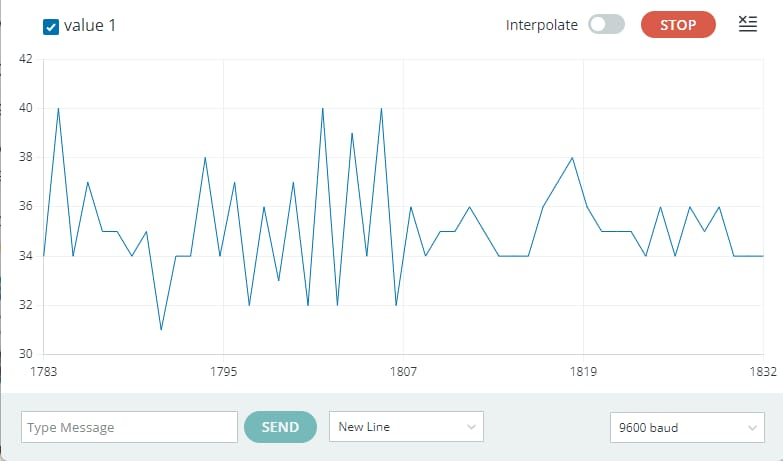
\includegraphics[width=12.8cm, keepaspectratio]{exp05_serial_plotter.jpeg}}\par\vspace{0.06cm}
{\small\textbf{Figure 5.1:} Arduino Serial Plotter waveform during dry soil baseline testing ($31 \le \text{ADC} \le 40$).}\par}

\newpage
% ==============================================================================
% PAGE 6: EXPERIMENT 06 - PIR MOTION SENSOR TELEMETRY
% ==============================================================================
\begin{center}
    {\large\bfseries Experiment 06: Interfacing PIR Motion Sensor with Arduino UNO}\\[0.08cm]
    {\normalsize\textbf{Passive Infrared Motion Detection \& Alert Telemetry --- Program Source Code \& Experimental Output}}
\end{center}
\vspace{-0.20cm}
\rule{\textwidth}{0.9pt}
\vspace{0.06cm}

\section*{1. Arduino C++ Source Code}
\begin{lstlisting}[style=bwCode, title={\textbf{Listing 6.1: Microcontroller Firmware for PIR Motion Sensing and Serial Event Telemetry.}}]
/*
 * Experiment 06: PIR Motion Sensor Interfacing with Arduino UNO
 * Hardware Pin Connections:
 *   - PIR Sensor OUT (O/P) -> Arduino Digital Pin 8 (Configured as INPUT)
 *   - PIR Sensor VCC       -> Arduino 5V Power Rail
 *   - PIR Sensor GND       -> Arduino Common Ground (GND)
 * Serial Baud Rate: 9600 bps | Sampling Interval: 100 ms
 */

const int motionPin = 8; // Digital input pin connected to PIR OUT

void setup() {
  pinMode(motionPin, INPUT); // Configure Pin 8 as digital input
  Serial.begin(9600);        // Initialize UART Serial Interface at 9600 Baud
}

void loop() {
  // Acquire digital logic state from PIR pyroelectric sensor module
  if (digitalRead(motionPin) == HIGH) {
    Serial.println("motion detected!");
  } else {
    Serial.println("No motion");
  }
  delay(100); // 100 ms sampling cycle delay to prevent buffer saturation
}
\end{lstlisting}

\vspace{0.06cm}
\section*{2. Experimental Output, Detection State Log \& Digital Waveforms}

\noindent
\textbf{A. Motion Detection Observation Table:}\par\vspace{0.06cm}
{\footnotesize
\setlength{\tabcolsep}{4.5pt}
\renewcommand{\arraystretch}{1.18}
\begin{tabularx}{\textwidth}{|c|p{4.6cm}|c|c|X|}
\hline
\textbf{\#} & \textbf{Human Target Motion State} & \textbf{Pin 8 Output} & \textbf{Serial Output} & \textbf{Hardware Alert Status} \\
\hline
1 & Quiescent / Idle Baseline & LOW ($0\,\text{V}$) & \texttt{No motion} & Quiescent Baseline (Sensor Armed) \\
2 & Active Hand Movement & HIGH ($5\,\text{V}$) & \textbf{\texttt{motion det.!}} & Motion Triggered ($T_{\text{hold}}$ Active) \\
3 & Continuous Motion Transit & HIGH ($5\,\text{V}$) & \textbf{\texttt{motion det.!}} & Retrigger Interval Extended \\
4 & Target Stationary State & LOW ($0\,\text{V}$) & \texttt{No motion} & Quiescent Baseline (Reset) \\
5 & Secondary Transit Cycle & HIGH ($5\,\text{V}$) & \textbf{\texttt{motion det.!}} & Motion Triggered ($T_{\text{hold}}$ Active) \\
\hline
\end{tabularx}
}

\vspace{0.20cm}

\noindent
\textbf{B. Serial Monitor Stream (9600 Baud):}\par\vspace{0.05cm}
\begin{lstlisting}[style=bwTerminal]
motion detected!
motion detected!
No motion
No motion
motion detected!
\end{lstlisting}

\vspace{0.18cm}

\noindent
\textbf{C. PIR Sensor Thermal Flux \& Digital Output Timing Waveform ($T_{\text{hold}}$):}\par\vspace{0.05cm}
{\centering
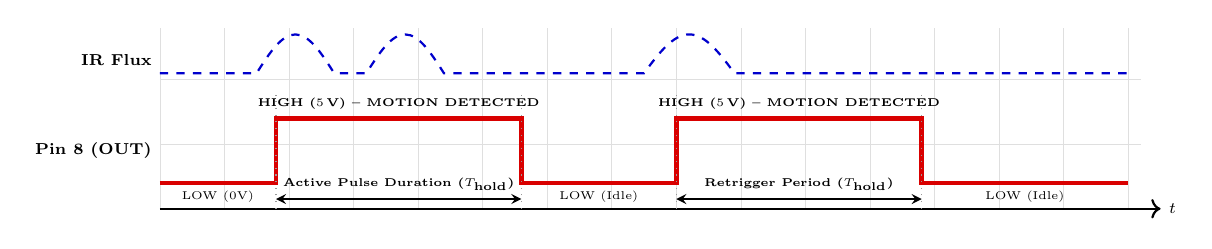
\begin{tikzpicture}[scale=0.82, every node/.style={transform shape}]
    \draw[step=1.0cm,gray!25,very thin] (0,0) grid (15.2,2.8);
    \draw[thick,->] (0,0) -- (15.5,0) node[right, font=\scriptsize] {$t$};
    
    % IR Heat Flux / Movement (Analogue stimulus)
    \draw[dashed, blue!80!black, thick] 
        (0,2.1) -- (1.5,2.1) 
        sin (2.1,2.7) cos (2.7,2.1) -- (3.2,2.1)
        sin (3.8,2.7) cos (4.4,2.1) -- (7.5,2.1)
        sin (8.2,2.7) cos (8.9,2.1) -- (15.0,2.1);
    \node[left, font=\scriptsize\bfseries] at (0,2.3) {IR Flux};

    % Digital Pin 8 Pulse (PIR Output)
    \draw[ultra thick, red!85!black] 
        (0,0.4) -- (1.8,0.4) -- (1.8,1.4) -- (5.6,1.4) -- (5.6,0.4) 
        -- (8.0,0.4) -- (8.0,1.4) -- (11.8,1.4) -- (11.8,0.4) -- (15.0,0.4);
    \node[left, font=\scriptsize\bfseries] at (0,0.9) {Pin 8 (OUT)};
    
    % Logic State labels
    \node[below, font=\tiny] at (0.9,0.4) {LOW (0V)};
    \node[above, font=\tiny\bfseries] at (3.7,1.42) {HIGH ($5\,\text{V}$) -- MOTION DETECTED};
    \node[below, font=\tiny] at (6.8,0.4) {LOW (Idle)};
    \node[above, font=\tiny\bfseries] at (9.9,1.42) {HIGH ($5\,\text{V}$) -- MOTION DETECTED};
    \node[below, font=\tiny] at (13.4,0.4) {LOW (Idle)};
    
    % Timing markers
    \draw[dotted, gray!80] (1.8,0) -- (1.8,1.8);
    \draw[dotted, gray!80] (5.6,0) -- (5.6,1.8);
    \draw[<->, >=stealth, black, semithick] (1.8,0.15) -- (5.6,0.15) node[midway, above, font=\tiny\bfseries] {Active Pulse Duration ($T_{\text{hold}}$)};
    
    \draw[dotted, gray!80] (8.0,0) -- (8.0,1.8);
    \draw[dotted, gray!80] (11.8,0) -- (11.8,1.8);
    \draw[<->, >=stealth, black, semithick] (8.0,0.15) -- (11.8,0.15) node[midway, above, font=\tiny\bfseries] {Retrigger Period ($T_{\text{hold}}$)};
\end{tikzpicture}\par\vspace{0.05cm}
{\small\textbf{Figure 6.1:} PIR sensor analog IR flux response and digital retrigger timing waveform ($T_{\text{hold}}$).}\par}

\end{document}
